%%%%%%%%%%%%%%%%%%%%%%%%%%%%%%%%%%%%%%%%%
% Arsclassica Article
% LaTeX Template
% Version 1.1 (10/6/14)
%
% This template has been downloaded from:
% http://www.LaTeXTemplates.com
%
% Original author:
% Lorenzo Pantieri (http://www.lorenzopantieri.net) with extensive modifications by:
% Vel (vel@latextemplates.com)
%
% License:
% CC BY-NC-SA 3.0 (http://creativecommons.org/licenses/by-nc-sa/3.0/)
%
%%%%%%%%%%%%%%%%%%%%%%%%%%%%%%%%%%%%%%%%%

%----------------------------------------------------------------------------------------
%	PACKAGES AND OTHER DOCUMENT CONFIGURATIONS
%----------------------------------------------------------------------------------------


\documentclass[
11pt, % Main document font size
a4paper, % Paper type, use 'letterpaper' for US Letter paper
oneside, % One page layout (no page indentation)
%twoside, % Two page layout (page indentation for binding and different headers)
headinclude,footinclude, % Extra spacing for the header and footer
BCOR5mm, % Binding correction
]{scrartcl}






\input{structure.tex} % Include the structure.tex file which specified the document structure and layout

\hyphenation{Fortran hy-phen-ation} % Specify custom hyphenation points in words with dashes where you would like hyphenation to occur, or alternatively, don't put any dashes in a word to stop hyphenation altogether

%----------------------------------------------------------------------------------------
%	TITLE AND AUTHOR(S)
%----------------------------------------------------------------------------------------

\title{\normalfont\spacedallcaps{MTH9899 Final Project Machine Learning}} % The article title

\author{Group x22\\ \spacedlowsmallcaps{ \small{Hongshan Chu, Yuchen Qi, Linwei Shang, ShengQuan Zhou} }} % The article author(s) - author affiliations need to be specified in the AUTHOR AFFILIATIONS block

\date{} % An optional date to appear under the author(s)

%----------------------------------------------------------------------------------------

\begin{document}



%----------------------------------------------------------------------------------------
%	HEADERS
%----------------------------------------------------------------------------------------

\renewcommand{\sectionmark}[1]{\markright{\spacedlowsmallcaps{#1}}} % The header for all pages (oneside) or for even pages (twoside)
%\renewcommand{\subsectionmark}[1]{\markright{\thesubsection~#1}} % Uncomment when using the twoside option - this modifies the header on odd pages
\lehead{\mbox{\llap{\small\thepage\kern1em\color{halfgray} \vline}\color{halfgray}\hspace{0.5em}\rightmark\hfil}} % The header style

\pagestyle{scrheadings} % Enable the headers specified in this block

%----------------------------------------------------------------------------------------
%	TABLE OF CONTENTS & LISTS OF FIGURES AND TABLES
%----------------------------------------------------------------------------------------

\maketitle % Print the title/author/date block

\setcounter{tocdepth}{2} % Set the depth of the table of contents to show sections and subsections only


\tableofcontents % Print the table of contents

%----------------------------------------------------------------------------------------
%	ABSTRACT
%----------------------------------------------------------------------------------------

\section*{Abstract} % This section will not appear in the table of contents due to the star (\section*)
In this project, we experimented several machine learning methods to predict stock returns from a set of features. A variety of measures including Pearson's correlation coefficient, Kendall's tau and Spearman's rho are used to preprocess data and select features. Preliminary predictive calculations are performed using linear regressions and tree-based methods and benchmarked by in-sample and out-of-sample $R^2$, coefficients of determination. Detailed calculations and parameter tuning are performed using \textit{Gradient Boosting Regression Trees}. In the training/testing process, a range of values $5\sim 15$ (bps) are reached for the out-of-sample $R^2$ from boosting trees, which is the method used in the submitted solution for the hold-out dataset, for which our model achieved an out-of-sample $R^2>20$bps.

\listoffigures % Print the list of figures

\listoftables % Print the list of tables




{\let\thefootnote\relax\footnotetext{* \textit{Baruch MFE}}}


%----------------------------------------------------------------------------------------

\newpage % Start the article content on the second page, remove this if you have a longer abstract that goes onto the second page

%----------------------------------------------------------------------------------------
%	INTRODUCTION
%----------------------------------------------------------------------------------------

\section{Overview of Dataset}
The training dataset contains 
\begin{itemize}[noitemsep]
\item $\sim$ 140,000 rows;
\item key: stock ID and a timestamp;
\item 27 features: 17 quantitative and 10 categorical;
\item A \textit{weight} column and an output column representing stock returns.
\end{itemize}
A few general guidelines are followed in this work:
\begin{itemize}[noitemsep]
\item Predictions are made based on the information contained in each row, without cross-row reference.
\item No time series modelling is explored, partly because the data points per stock ID along time axis are inhomogeneous and incomplete.
\item No stock-specific modeling is explored given that the data points per stock ID are inhomogeneous and incomplete.
\item Timestamp information is used only for dividing the dataset into training set and test set.
\item Weighted $R^2$ is used as the final benchmark.
\end{itemize}

\section{Data Preprocessing}
The provided dataset is divided into two parts according to timestamp:
\begin{itemize}[noitemsep]
\item The first 2/3 are used for training and testing;
\item The remaining 1/3 are reserved for a production run.
\end{itemize}
A series of split points are chosen to divide the first 2/3 of the complete dataset into two parts:
\begin{itemize}[noitemsep]
\item The first part for training;
\item The second part for testing.
\end{itemize}
Note that, the training set always pre-dates the test set to avoid look-ahead bias.

\subsection{Selection of Quantitative Features}

Not all features are significantly relevant in predicting the output. We perform a preliminary data cleaning procedure to select relevant features before
running any machine learning algorithm of prediction. Two tests are performed to select \underline{quantitative} features:
\begin{itemize}[noitemsep]
\item Pearson correlation coefficient:
$$
\rho_{xy} = \frac{\text{Cov}(x,y)}{\sqrt{\text{Var}(x)\text{Var}(y)}},
$$
which measures the univariate linear relationship between a feature and the output.
\item Kendall's rank correlation coefficient, also known as Kendall's $\tau$:
$$
\tau_{xy} = \mathbb{P}[(x_1 - x_2)(y_1 - y_2)>0] - \mathbb{P}[(x_1 - x_2)(y_1 - y_2)<0],
$$
which measures the imbalance between the number of concordant pairs and the number of discordant pairs.
\item Spearman's rank correlation coefficient, also known as Spearman's $\rho$:
$$
\varrho_{xy} = 3 \left\{ \mathbb{P}[(x_1-x_2)(y_1-y_3)>0] -  \mathbb{P}[(x_1-x_2)(y_1-y_3)<0]\right\},
$$
which measures the difference of the probability of concordance and the probability of discordance for the vectors of random variables $(x_1,y_1)$ and $(x_2,y_3)$.
\end{itemize}
with respect to the training set of output data, based on the criterion that the $p$-value for correlation coefficients being less than $3\%$. Kendall's $\tau$ and Spearman's $\rho$ are able to capture nonlinear relationships.\\
\newline
The results are remarkably consistent in that all three measures of correlation with output select the same list of quantitative features for the training set:

\begin{table*}[ht!]
	\footnotesize
	\center
	\begin{tabular}{lrrrrrrrrr}  
		\toprule
		Feature & Pearson & $p$-value & Kendall's $\tau$ & $p$-value & Spearman's $\rho$ & $p$-value  \\
		\midrule		
		x0 & 	$-0.019$ & $10^{-6}$	&	$-0.013$ & $10^{-6}$	& $-0.019$	&	$10^{-6}$ \\
		x17 & $+0.016$	& $10^{-5}$	&	$+0.009$ & $10^{-3}$	& $+0.013$	&	$10^{-3}$ \\
		x22 & $+0.026$	& $10^{-11}$	&	$+0.014$ & $10^{-7}$	&	$+0.020$ &	$10^{-7}$ \\
		x49 & $+0.015$	& $10^{-4}$	&	$+0.009$ & $10^{-4}$	& $+0.013$	&	$10^{-4}$ \\
		x53 & $+0.018$	& $10^{-6}$	&	$+0.012$ & $10^{-6}$	& $+0.018$	&	$10^{-6}$ \\
		x61 & $-0.009$	& $0.03$	&	$-0.009$ & $10^{-3}$	& $-0.013$	&	$10^{-4}$ \\
		\bottomrule
	\end{tabular}
	\caption{\label{corr} Correlation measure of the selected list of quantitative features with respect to the output and the associated statistical
	significance test.} 
\end{table*}

In the submitted solution based on \textit{Gradient Boosting Regression Trees}, all six features listed above \{x0, x17, x22, x49, x53, x61\} are chosen as input features.

\subsection{Treatment of Categorical Features}
A similar set of tests on correlation coefficients are performed on \underline{categorical} features treated as ordinal numbers, which yields the following results:\\
\begin{table*}[ht!]
	\footnotesize
	\center
	\begin{tabular}{lrrrrrrrrr}  
		\toprule
		Feature & Pearson & $p$-value & Kendall's $\tau$ & $p$-value & Spearman's $\rho$ & $p$-value  \\
		\midrule
		x2 & $-0.038$	& $10^{-22}$	&	$-0.026$ & $10^{-21}$	& $-0.037$	&	$10^{-21}$ \\
		x6 & $-0.014$	& $10^{-4}$	&	$-0.007$ & $0.02$	&	$-0.010$ &	$0.01$ \\
		x30 & 	$+0.020$ & $10^{-7}$	&	$+0.014$ & $10^{-6}$	& $+0.018$	&	$10^{-6}$ \\
		x46 & $+0.026$	& $10^{-11}$	&	$+0.018$ & $10^{-10}$	& $+0.026$	&	$10^{-10}$ \\
		x51 & $+0.017$	& $10^{-5}$	&	$+0.011$ & $10^{-4}$	& $+0.015$	&	$10^{-4}$ \\
		\bottomrule
	\end{tabular}
	\caption{\label{corr} Correlation measure of the selected list of categorical features (treated as ordinal numbers) with respect to the output and the associated statistical	significance test.} 
\end{table*}\\
A selected list of categorical features are treated as
\begin{itemize}[noitemsep]
\item ordinal numbers; or
\item one-hot dummy variables.
\end{itemize}

In the submitted solution based on \textit{Gradient Boosting Regression Trees}, four categorical features \{x6, x30, x46, x51\} listed above, treated as ordinal numbers, are chosen as input features, excluding x2. Although feature x2 exhibits high correlation with respect the output, its behavior varies over time and does not help improve the out-of-sample prediction according to our experiments.

\subsection{Period-by-Period Correlations}
An investigation into the the evolution of features with respect to the output over time is performed by dividing the whole dataset into 9 chronologically ordered
periods.\\
\begin{table*}[ht!]
\small
\center
\begin{tabular}{lrrrrrrrrrrr}  
\toprule
Period & x0 & x17&	x22 	& x49	& x53 	 &	x61	 &			x30 &		x46 &		x51\\
\midrule
1 & 	-.013 & .007 & 	.018		& 	.014	& 	.022		& 	.008	& 		.005	& 	.027	& 	.003\\
2 & 	-.029  & .014 & 	.020	& 	.019	& 	.010			& 	-.009		& 	.012	& 	.020	& 	-.007\\
3 & 	-.027 & .021 & 	.015	& 	.006	& 	.016			& 	-.014		& 	-.002	& 	.014	& 	-.027\\
4 & 	-.006 & .018 & 	.045	& 	.017	& 	.025			& 	-.021		& 	.017	& 	.032	& 	-.002\\
5 & 	-.007  & .016 & 	.044	& 	.012	& 	.009			& 	-.002		& 	.019	& 	.033	& 	-.009\\
6 & 	-.014 & .009& 	.009 	& 	.017	& 	.012			& 	-.008		& 	-.0004	& 	.032	& 	.0005\\
7 & 	-.008 & .045 & 	.045	& 	.008	& 	.024			& 	-.004	& 	-.008		& 	.007	& 	-.003\\
8 & 	-.009 & .015 & 	.021		& 	.012	& 	.011		& 	.003	& 	-.009		& 	-.012	& 	-.003\\
9 & 	-.016 & .021 & 	.019	& 	-.010	& 	.006			& 	.004	& 	-.016		& 	.002	& 	-.013\\
\bottomrule
\end{tabular}
	\caption{\label{corr} Pearson correlation measure of a selected list of features with respect to the output over 9 successive time periods.} 
\end{table*}\\
It is observed that the correlations of most quantitative features with respect to the output are stable over time, except for x49 and x61 near the end of
the time horizon of the provided dataset, as shown in Figure \ref{corr}. One possible cause of this phenomena could be a market regime shifting and would help explain a decrease in out-of-sample $R^2$ when the ratio between the training set size and the test set size grows high, to be discussed in a later section. 
\begin{figure}[ht!]
\centering
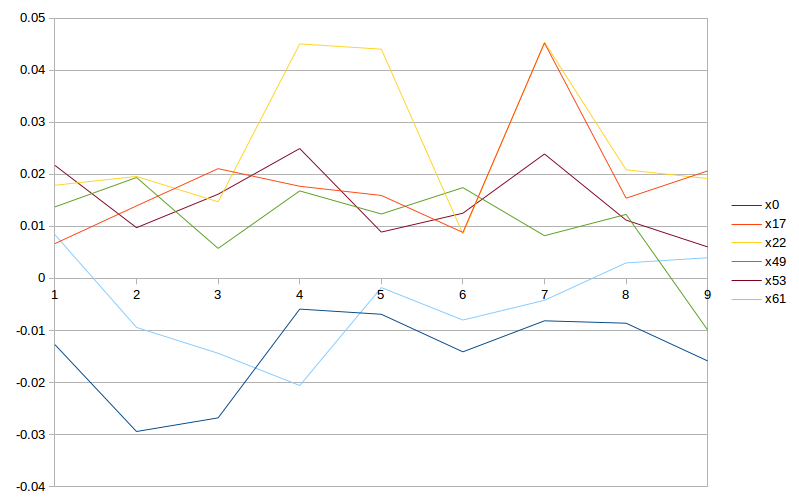
\includegraphics[width=12.4cm, height=6cm]{corr} 
\caption{Evolution of the univariate correlation coefficients of 6 selected quantitative features with respect the output $y$ over 9 successive time periods. It's observed that the feature x49 and x61 change their signs approaching the end of the time horizon.}\label{corr}
\end{figure}


\subsection{Data Cleaning: Removal of Outliers}\label{outlier}
Outliers observed in features and outputs in the \underline{training set} are removed to reduce the likelihood of overfitting:
\begin{itemize}[noitemsep]
\item Remove all data rows with output $|y|>0.05$. The threshold chosen for $y$ is based on an examination of the sample distribution drawn from the provided data, as show in Figure \ref{hist}.
\item Remove all data rows that have outliers in at least one column, based on the criterion $z$-score>3.
\end{itemize}
\begin{figure}[ht!]
\centering
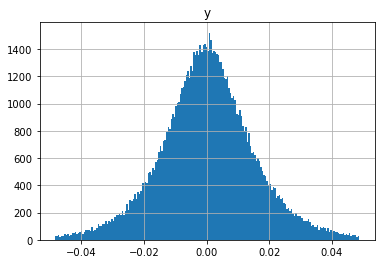
\includegraphics[width=12cm, height=5.9cm]{hist} 
\caption{Sample distribution of the output $y$. Number of bins=200.}\label{hist}
\end{figure}
 
%
 
\newpage 
%----------------------------------------------------------------------------------------
%	METHODS
%----------------------------------------------------------------------------------------

\section{Methods}
Several standard machine learning methods are experimented including
\begin{itemize}[noitemsep]
\item Linear regressions:
\begin{itemize}[noitemsep]
	\item OLS;
	\item Ridge;
	\item Lasso.
\end{itemize}
\item Tree-based methds:
\begin{itemize}[noitemsep]
	\item Random forest;
	\item Boosting trees.
\end{itemize}
\end{itemize}
Preliminary calculations are preformed with linear regressions and tree-based methods to get an order of magnitude estimate of the out-of-sample $R^2$ attainable. Then we focus on the method of \textit{Gradient Boosting Regression Trees} with detailed parameter tuning to improve the results, on which the final submitted solution is based.\\
\newline
The software package used in this work is \textit{scikit-learn}.

\subsection{Linear Regressions}

\textit{Weighted Least Square} are tested using all features and the selected features. As shown in Table \ref{linearregression}, using the full set of 
features causes significant overfitting, giving rise to high positive in-sample $R^2$ as well as high negative out-of-sample $R^2$. Using the selected list
of features fixes the problem of overfitting, giving rise to reasonable estimates for the out-of-sample $R^2\sim 7$bps.\\
\begin{table}[ht!]
\center
	\begin{tabular}{lrrrrrrrrr}  
		\toprule
		Method & Feature & In-Sample $R^2$(bps) & Out-of-Sample $R^2$(bps) \\
		\midrule
	    OLS & all  & $+47.20$	& $-23.37$	 \\
		OLS & selected  & $+6.28$	& $+7.33$	 \\
		Ridge & selected  & 	$+3.91$ & $+7.19$	  \\
		Lasso & selected  & $+3.10$	& $+7.01$	 \\
		\bottomrule
	\end{tabular}
	\caption{Results on in-sample and out-of-sample $R^2$ using linear regresion methods.}\label{linearregression}
\end{table}\\
Both \textit{Ridge Regression} and \textit{Lasso Regression} give a similar estimate for out-of-sample $R^2\sim 7$bps as the ordinary (weighted) least square and slightly reduced in-sample $R^2$.\\
\newline
The above results show that regularization penalty does not significantly improve the ordinary least square for out-of-sample prediction. We interpret this observation as an indication of the underfitting nature of the linear regression methods, which, however, give us a basic understanding about how good our selected features are.

\subsection{Tree-Based Methods}
Tree-based methods are known to be less likely to underfit and serves as the primary tool in this work. We first summarize the results in Table \ref{treemethods} and give detailed discussion in the following sections.

\begin{table}[ht!]
\center
	\begin{tabular}{lrrrrrrrrr}  
		\toprule
		Method & In-Sample $R^2$(bps) & Out-of-Sample $R^2$(bps) \\
		\midrule
	    Random Forest  & $+5.3$	& $+3.9$	 \\
		Boosting Trees (2:1) & $+10$	& $+4.7$	 \\
		Boosting Trees (3:1)  & $+10$	& $+12.7$	 \\
		\bottomrule
	\end{tabular}
	\caption{Results on in-sample and out-of-sample $R^2$ using tree-based methods, including random forest and boosting trees. For the method of boosting trees, two results are reported with train/test ratio 2:1 and 3:1.}\label{treemethods}
\end{table}

\subsubsection{Random Forest}
\textit{Random Forest} is a substantial modification of bagging that builds a large collection of de-correlated trees, each of the relevant variables getting their turn to be the primary split, and then the ensemble averaging redcues the contribution of any individual variable. There exists a claim that random forests \textit{cannot overfit} the data. On many problems the performance of random forests is very similar to boosting trees experimented in Section \ref{boostingtrees}, but they are simpler to train and tune.\\
\newline
An image of a (illustrative) random forest is shown in Figure \ref{rf} as randomly behaving trees growing in parallel.
\begin{figure}[ht!]
\centering
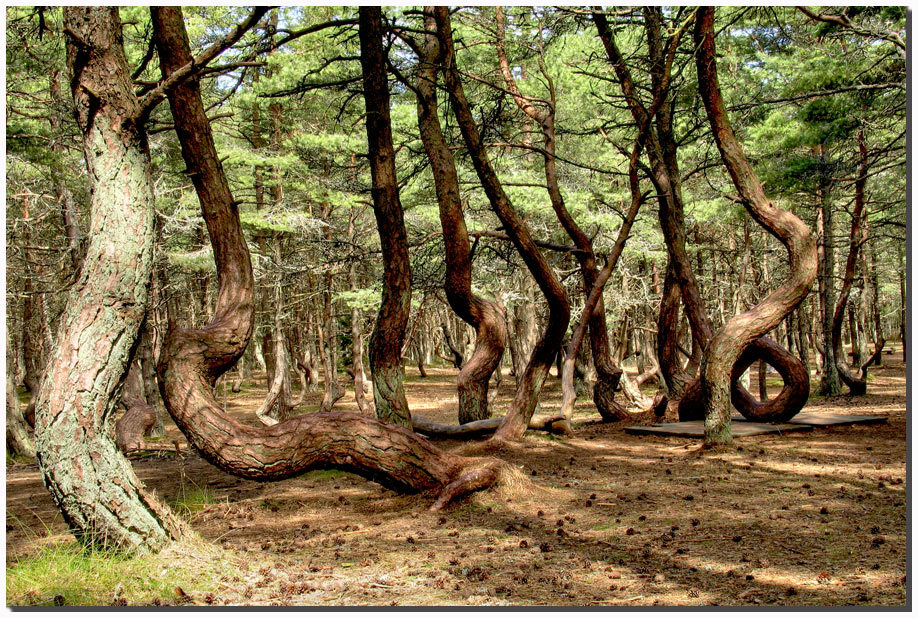
\includegraphics[width=10cm, height=5cm]{rf.jpg} 
\caption{An illustration of random forest (unknown location).}\label{rf}
\end{figure}


The primary set of parameters to be tuned for the random forest regression are
\begin{itemize}[noitemsep]
	\item Number of trees (=40);
	\item Maximum depth per tree (=None);
	\item Minimum number of samples per leaf (=8000);
	\item Minimum number of samples for a node to split (=8000);
	\item Whether bootstrap samples are used when building trees (=True),
\end{itemize}
where the parameters chosen for the results reported in Table \ref{treemethods} are shown in parenthesis. A rule-of-thumb wisdom is that using full-grown trees seldom costs much and results in one less tuning parameter in random forests.\\
\newline
The results in Table \ref{treemethods}
shows that, without an in-depth tuning of parameters, the method of random forest gives an estimate of in-sample and out-of-sample $R^2$ on the order of a few basis points and underperforms the linear regression methods.


\subsubsection{Gradient Boosting Trees}\label{boostingtrees}
Quantitatively speaking, for least square type of loss function, each tree in the hierarchy fits the residual from the previous tree. Pictorially, boosting trees can be imagined as a set of trees growing one on top of an other, as illustrated in Figure \ref{boosting}:

\begin{figure}[ht!]
\centering
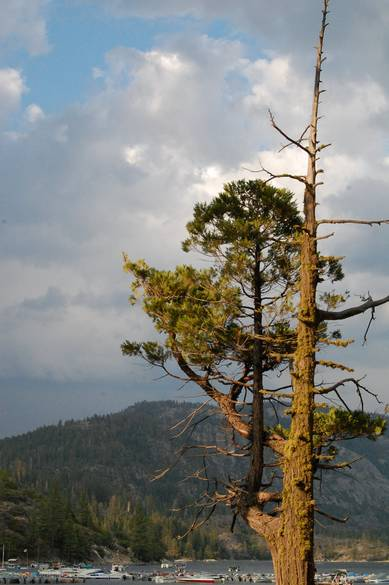
\includegraphics[width=6.8cm, height=8.5cm]{boosting.jpg} 
\caption{Tree on a tree. Pinecrest, CA. An illustration of the method of boosting trees, where one tree grows on the top of another tree, forming a boosting hierarchy. Compare the aspect ratio of this Figure with Figure \ref{rf} to get an idea of how the trees are growing.}\label{boosting}
\end{figure}

The method of boosting trees has a larger number of parameters to tune than random forests:
\begin{itemize}[noitemsep]
	\item \underline{Number of trees}, or the number of boosting stages to perform. In the submitted solution, we chose $M=75$;
	\item \underline{Size of each tree} ($J$). Experience so far indicates that $4\le J\le 8$ works well in the context of boosting, with results being fairly
	insensitive to particular choices in this rangge. We have fine-tuned the value for $J$ by trying different values and choosing the one that produces
	the lowest $R^2$ on average on a validation sample. In the submitted solution, we chose $J=6$.
	\item \underline{Learning rate}, also known as the shrinkage parameter $\nu$, controlls the learning rate of the boosting procedure. Small values of $nu$ result in larger
	training risk for the same number of iterations $M$. Empirical evidence have been found that smaller values of $\nu$ favor better test error, and require correspondingly larger values for $M$. In the submitted solution, we chose $\nu=0.017$.
	\item \underline{Subsampling} ($\eta$). With stochastic gradient boosting, at each iteration, we sample a fraction $\eta$ of the training observations (without replacement), and grow the next tree using that subsample. A typical valuefor $\eta$ can be $\frac{1}{2}$. In the submitted solution, we chose $\eta=1$, i.e., no subsampling.
	\item \underline{Minimum number of samples per leaf} (=500 chosen in the submitted solution).
\end{itemize}
In summary, we have basically four parameters $M,J,\nu,$ and $\eta$. Typically some early explorations determine suitable values for $J,\nu$, $\eta$, leaving $M$ as the primary parameter. In this project, we performed a detailed grid-search to fine-tune the set of parameters for the method of boosting trees. We obtained progressively better results as we tune the parameters, a sample result is shown in Table \ref{treemethods}.


\subsection{A Closer Look at Data Split}

In this section, we take a closer look at the performance of the method of boosting trees as we split the data into training set and test set differently. It is an invariant that the training set always pre-dates the test set to avoid look-ahead bias. In Table \ref{split}, we tabulate the results on the dependence of the out-of-sample $R^2$ on the splitting ratio defined as
$$
\frac{\text{Size of Training Set}}{\text{Size of Test Set}}.
$$
An interesting observation from the tabulated results is that the out-of-sample $R^2$ does not change monotonically with the splitting ratio. When the training set is smaller in size than the test, the out-of-sample $R^2$ are negative in our experiments (not tabulated). As the splitting ratio grows from $1$ to $4$, the out-of-sample $R^2$ grows accordingly and reaches a maximum at a splitting ratio $3$ or $4$. As the splitting ratio grows further, out-of-sample $R^2$ declines. This  pattern could indicate the existence of a change in the underlying market regime approaching the end of the provided dataset. Another explanation is that the out-of-sample $R^2$, which is itself a random variable, simply has a large variance resulting from the small size of test dataset. \\
\newline
A question that naturally arises in this context and deserves further invesigation is that, given the fact that the hold-out dataset consists of 25\% of the complete dataset, whether we should the train the model with a fixed ratio between the training set size and test set size, or we should choose a fixed size for the training set. Or given a certain window length of predicting horizon, does the market keep a proportional length of memory or a fixed length of memory? 

\begin{table}[ht!]
\center
\small
	\begin{tabular}{lrrrrrrrrr}  
		\toprule
		Train \# / Test \# & $R^2$(bps) No Outlier Removal &  $R^2$(bps) Outlier Removal \\
		\midrule
	    1:1 & \color{red}{$+3$}	& \color{red}{$+4$}	 \\
	    2:1 & \color{red}{$+4$}	& \color{red}{$+5$}	 \\
	    3:1 & \color{red}{$+15$}	& \color{red}{$+13$}	 \\
	    4:1 & \color{red}{$+15$}	& \color{red}{$+13$}	 \\
	    5:1 & \color{red}{$+7$}	& $\sim 1$	 \\
	    6:1 & $\sim 1$	& $-5$	 \\
	    7:1 & $-2$	& $-3$	 \\
	    8:1 & $-1$	& $-2$	 \\
		\bottomrule
	\end{tabular}
	\caption{The dependence of out-of-sample $R^2$ on splitting ratio of the dataset. For experimenting purposes, we explored two cases: including an excluding the outlier removal procedure described in Section \ref{outlier}. }\label{split}
\end{table}


\section{Conclusion and Outlook}
\begin{itemize}[noitemsep]
\item In this project, the methods of linear regressions, random forests, and gradient boosting trees are experimented to predict stock returns from a given set of features.
\item With a series of procedures including feature selection and data cleaning, a range of values $5\sim 15$(bps) are reached for the out-of-sample $R^2$ for boosting trees in the training/testing process. 
\item The submitted solution is based on \textit{Gradient Boosting Regression Trees}, which worked best during our exploration. In the hold-out dataset,  our model achieved an out-of-sample $R^2>20$bps.
\item As a future enhancement, a mixture of models, for example, boosting trees combined with random forests, is expected to improve the performance.
\end{itemize}

%----------------------------------------------------------------------------------------
%	BIBLIOGRAPHY
%----------------------------------------------------------------------------------------

\renewcommand{\refname}{\spacedlowsmallcaps{References}} % For modifying the bibliography heading

\bibliographystyle{unsrt}

\bibliography{sample.bib} % The file containing the bibliography

%----------------------------------------------------------------------------------------

\end{document}